\chapter{Elementi di Ottica Diffrattiva e Fasci Gaussiani}
\graphicspath{{./cap_3/images/}}

\section{Equazioni d'onda parassiale}
Consideriamo un'onda e.m. monocromatica di frequenza $\w$ in vuoto.\\
Detto:
\begin{equation*}
\*E(x,y,z,t) = \frac{1}{2} \left[\*E(x,y,z) e^{i\omega t} + c.c.\right]
\end{equation*}
il campo elettrico dell'onda, è noto che $\widetilde{E}(x,y,z)$ soddisfa l'equazione di Helmholtz:
\begin{equation}\label{eq: 1}
\nabla^2 \widetilde{E} + k^2 \widetilde{E} = 0 \quad \text{con } \quad k \equiv \frac{\omega}{c}
\end{equation}
Una soluzione semplice, corrispondente ad un'onda piana è $\widetilde{E} = E_x(z)\hat{u}_x$ linearmente polarizzata lungo $x$ che si propaga nella direzione $z$, con:
\begin{equation*}
E_x(z) = E_0 e^{-ikz}
\end{equation*}
Vogliamo cercare una soluzione dell'equazione \eqref{eq: 1}, che approssimi l'onda piana progressiva che si propaga lungo $z$ ma che trasporti potenza finita. Facciamo l'Ansatz:
\begin{equation*}
\widetilde{E} = u(x,y,z) e^{-i k z} \hat{u}_x
\end{equation*}
funzione di $z$ (lei e le sue derivate) lentamente variabile su scala spaziale $\lambda = \frac{2\pi}{k}$.
cioè
\begin{equation*}
\left| \frac{\partial u}{\partial z} \lambda \right| << |u| \quad \left| \frac{\partial^2 u}{\partial z^2} \lambda \right| << \left|\frac{\partial u}{\partial z}\right|
\end{equation*}
(SVEA: slowly varying envelop approximation). Sostituendo l'Ansatz (2) nella \eqref{eq: 1} e usando la SVEA ottengo:
\begin{equation*}
\frac{\partial^2}{\partial z^2} (u e^{ikz)} + (\nabla_t^2 u) e^{-ikz} = 0
\end{equation*}
dove ho posto:
\begin{equation*}
\nabla_t^2 \equiv \frac{\partial^2}{\partial x^2}
\end{equation*}
\begin{equation*}
\frac{\partial^2 u}{\partial z^2} e^{-ikz} -k^2 u e^{-ikz} - 2ik \frac{\partial}{\partial z} e^{-ikz} + (\Delta_t^2 u) 
\end{equation*}
cioè:
\begin{equation*}
\frac{\partial^2}{\partial z^2}
\end{equation*}
cioè $u(x,y,z)$ soddisfa l'equazione parassiale dell'onda:
\begin{equation*}
i\frac{\partial}{\partial z} = \frac{1}{2k} \nabla_t^2 u
\end{equation*}
La soluzione banale $u = E_0$ costante è il limite d'onda piano.\\
L'intensità media (sul ciclo attivo) dell'onda è:
\begin{equation*}
I = <|\*E \times \*H|> = ... = \frac{1}{2} \varepsilon_0 c_0 |u(x,y,z)|^2
\end{equation*}
per cui la potenza $P$ trasportata dall'onda vale:
\begin{equation*}
P = \iint_{-\infty}^{+\infty} I(x,y,z) dxdy
\end{equation*}
cioè:
\begin{equation*}
P = \frac{1}{2} \varepsilon_0 c_0 \iint_{-\infty}^{+\infty} dxdy |u(x,y,z)|^2
\end{equation*}
\subsubsection{Esercizio:}
Dimostro che 
\begin{equation*}
\frac{d}{dz} \iint_{-\infty}^{+\infty} (uu^*) dxdy \equiv 0
\end{equation*}
cioè la potenza $P$ dell'onda non varia con $z$ (ovvio: i fotoni dell'onda non vengono né creati né distrutti).

\textbf{Nota} Ho supposto che $\*E // \hat{u}_x$ e $\*B // \hat{u}_y$, il ché è vero solo per un'onda piana. Per un'onda non piana, questo è vero solo approssimativamente. Perché? Violo la I equazione di Maxwell $div \*E = 0$ cioè $\frac{\partial E_x}{\partial x} = 0$. Ma $E_x = (u(x,y,z) e^{-ikz}$  implica $\frac{\partial u}{\partial x} = 0$, derivante dalla II equazione di Maxwell, $div \*B = 0$, avrei $\frac{\partial u}{\partial y} = 0$. In definitiva $\frac{\partial u}{\partial x} = \frac{\partial u}{\partial y} = 0$, $\nabla_t^2 u = 0 \rightarrow \frac{\partial u}{\partial x} = 0$, $u = E_0$. A rigore, la soluzione parassiale (SVEA) a potenza finita sono quasi TEM.\\
\\
La soluzione più generale dell'equazione d'onda parassiale:
\begin{equation*}
i \frac{\p \psi}{\p z} = \frac{1}{2k} \left(\frac{\p^2 \psi}{\p x^2} + \frac{\p^2 \psi}{\p y^2} \right)
\end{equation*}
è data dall'integrale di KHF (Kirchhoff-Huygens-Fresnel)
%disegno
\begin{equation*}
u(x,y,z) = \frac{i}{\l (z - z_1)} \iint_{-\infty}^{+\infty} dx_1dy_1 u(x_1,y_1,z_1) e^{-\frac{ik}{2(z-z_1)} \left[ (x-x_1)^2 + (y-y_1)^2 \right]}
\end{equation*}

\subsection{Propagazione di un'onda monocromatica parassiale in un sistema ottica gaussiano}
Considero un'onda monocromatica con frequenza $\w$ parassiale che si propaga in un sistema ottico (S.O.) gaussiano (cioè con superfici riflettenti/rifrangenti sferiche) con asse ottico $z$.\\
La propagazione dell'onda si descrive in due modi:
\begin{equation*}
\begin{cases}
\text{limite dell'ottica geometrica: matrici (a raggi) ABCD}\\
\text{ottica ondulatoria: integrale di KHF generalizzato.}
\end{cases}
\end{equation*}
\textbf{Osservazioni:}\\
\begin{enumerate}
\item Matrici ottiche elementari
\begin{enumerate}
\item Propagazione libera
\[
\begin{bmatrix}
1	&	L\\
0	&	1
\end{bmatrix}
\]
\item Lente sferica sottile
\[
\begin{bmatrix}
1	&	0\\
-\frac{1}{f}	&	1
\end{bmatrix}
\]
con $f > 0$ se lente convergente e viceversa
\item Riflessione da specchio sferico
\[
\begin{bmatrix}
1	&	0\\
-\frac{2}{R}	&	1
\end{bmatrix}
\]
con $r >0$ se il raggio coincide dalla parte concava e viceversa.
\end{enumerate}
\item Matrici ABCD di s.o. composto. Se il raggio luminoso si propaga da $\alpha \rightarrow \beta$ incontrando una successione di S.O. elementari di matrici $M_1, M_2 ... M_N$, la matrice $M$ di propagazione da $\alpha$ a $\beta$ vale:
\begin{equation*}
M = M_NM_{N-1}...M_1
\end{equation*}
\item Il determinante della matrice ABCD vale:
\begin{equation*}
AD - BC = \frac{n_2}{n_1}
\end{equation*}
dove $n_1$ e $n_2$ sono gli indici di rifrazione dei mezzi in ingresso (piano $\alpha$) e uscita (piano $\beta$).
\end{enumerate}

\section{Fasci gaussiani I: definizione del fascio gaussiano fondamentale $TEM_{00}$ e legge ABCD}
I fasci gaussiani sono una famiglia di onde monocromatiche parassiali che, propagandosi in un arbitrario s.o. gaussiano (in particolare in propagazione libera cioè in vuoto) restano \textit{funzionalmente invarianti}. Il fascio gaussiano più semplice, detto fondamentale, è indicato con la sigla $TEM_{00}$.\\
Facciamo questo Ansatz:
%disegno
nel piano $z = z_1$, considero la distribuzione $u(x_1,y_1,z_1) = u_0 e^{-\frac{k(x_1^2 + y_1^2)}{2 q_1}}$ dove $q_1$ è un numero complesso detto parametro Q del fascio gaussiano. La condizione che il fascio trasporti potenza finita, e che:
\begin{equation*}
\iint_{-\infty}^{+\infty} dx_1 dy_1 |u(x_1,y_1,z_1)|^2 < \infty
\end{equation*}
ciò implica necessariamente la condizione $\Im{\frac{1}{q_1}} < 0$ o, che è lo stesso, $\Im{q_1} > 0$. Sostituendo l'Ansatz (1) nell'integrale generalizzato di KHF, si ottiene:
\begin{equation*}
u(x,y,z) = \frac{i}{\l B} \iint_{-\infty}^{+\infty} dx_1 dy_1 u(x_1,y_1,z_1) e^{\frac{ik}{2B} [A (x_1^2 + y_1^2) + D(x^2 + y^2) -2xx_1 - 2yy_1]}
\end{equation*}
\begin{equation*}
u(x,y,z) = \frac{u_0}{A + \frac{B}{q_1}} e^{-\frac{ik(x^2 + y^2)}{2q(z)}}
\end{equation*}
dove ho posto:
\begin{equation*}
q(z) = \frac{Aq_1 + B}{Cq_1 + D}
\end{equation*}
legge ABCD di propagazione del parametro complesso del fascio gaussiano.
La distribuzione gaussiana (1) si propaga in un arbitrario s.o. rimanendo funzionalmente invariante. Propagare un fascio gaussiano equivale, in sostanza, a propagare secondo la legge ABCD il suo parametro Q.\\
\subsubsection{Significato fisico di $q$} Introduco l'Ansatz:
\begin{equation*}
\frac{1}{q} = \frac{1}{R} - i\frac{\l}{\pi w^2}
\end{equation*}
con $\mathfrak{Re}$ e $\w$ reali e dimensionalmente lunghezze.
Per capire il significato fisico di $\Re$ e $\w$, osserviamo che:
\begin{equation*}
u(x,y,z) \propto e^{-i\frac{(x^2 + y^2)}{2q(z)}} \underbrace{=}_\text{Ansatz (3) non si dimostra} e^{-i\frac{(x^2 + y^2)}{2\Re(z)}} e^{-i\frac{(x^2 + y^2)}{w^2(z)}}
\end{equation*}
per cui la distribuzione trasversale di intensità del fascio, al piano $z = z$ vale:
\begin{equation*}
I(x,y,z) = \frac{1}{2} \varepsilon_0 c_0 |u|^2 \propto e^{-\frac{2 (x^2 + y^2)}{w^2(z)}}
\end{equation*}
cioè la distribuzione è gaussiana con dimensione di macchia \textit{spot size} $w$.
Per capire il significato di $R = R(z)$, calcoliamo le superfici equifase (fronti d'onda) dell'onda e.m.\\
Ricordando:
\begin{equation*}
\widetilde{E}(x,y,z) = u(x,y,z) e^{-ikz}
\end{equation*}
e
\begin{equation*}
E(x,y,z,t) = \frac{1}{2} \left[\widetilde{E} e^{-ikt} + c.c.\right] = \frac{1}{2} \left[u e^{i\omega t-ikt} + c.c.\right]
\end{equation*}
posso scrivere:
\begin{equation*}
E(x,y,z) = \frac{1}{2} \left[|u| e^{i\phi-ikt + i\omega t} + c.c.\right]
\end{equation*}
con $\phi$ fase di $u$. Le superfici equifase, per definizione
\begin{equation*}
\phi - kz = costante
\end{equation*}
Ma $\phi = -\frac{k (x^2 + y^2)}{2R}$, per cui le superfici equifase del fascio gaussiano sono:
\begin{equation*}
-\frac{k (x^2 + y^2)}{2R} - kz = costante
\end{equation*}
cioè:
\begin{equation*}
z = - \frac{x^2 + y^2}{2R} + costante'
\end{equation*}
ovvero, le superfici equifase (trascurando la dipendenza di $R$ da $z$ che è lenta su scala della $l$) sono paraboloidi di rotazione attorno all'asse $z$ e $R$ è il raggio della sfera osculatrice del paraboloide nel suo vertice.
%disegno
Si noti che se $R > 0$ la concavità del paraboloide è discorde con l'asse $z$ (come in figura), mentre se $R < 0$ la concavità è concorde con il verso di $z$. $R$ è detto raggio di curvatura del fascio gaussiano al piano $z$.\\
Si noti che al variare di $z$, sia $w$ che $R$ variano.

\section{Fasci gaussiani II: propagazione libera del fascio gaussiano fondamentale}
Studiamo la propagazione libera di un fascio gaussiano (cioè propagazione in vuoto).
%disegno
La matrice ABCD da $\alpha$ a $\beta$ vale
\[
\begin{bmatrix}
A	&	B\\
C	&	D
\end{bmatrix} =
\begin{bmatrix}
1	&	z - z_1\\
0	&	1
\end{bmatrix}
\]
per cui dalla legge ABCD ho:
\begin{equation*}
q(z) = \frac{Aq_1 + B}{Cq_1 + D} = q_1 + z - z_1
\end{equation*}
con $\Im{q_1} > 0$. Senza ledere di generalità, posso assumere $q_1$ puramente immaginario. Inoltre, posso assumere $z_1 = 0$. In $z = z_1 = 0$ ho dunque $q(z) = q_1 = iz_R$ dove $z_R$ è detto parametro (o lunghezza) di Rayleigh del fascio gaussiano. Si noti che, dire che in $z = z_1 = 0$ $q = q_1$ è puramente immaginario, equivale a dire che il fronte di fase del fascio in $z = 0$ è piano, cioè $R(z=0) = \infty$.\\
Pertanto:
\begin{equation*}
q(z) = z + iz_R \qquad \text{propagazione del parametro q libero (su $z=0$ ho fronte di fase piano cioè $R=\infty$)}
\end{equation*}
\\
Calcoliamo ora come evolvono $w(z)$ e $R(z)$.\\
Dall'Ansatz:
\begin{equation*}
\frac{1}{q(z)} = \frac{1}{R(z)} -i\frac{\l}{\pi w^2(z)} = \frac{1}{z + iz_R} = \frac{z - iz_R}{z^2 + z_R^2}
\end{equation*}
uguagliando per parti $\Re$ e $\Im$ dei due termini sottolineati ottengo
\begin{equation*}
\frac{1}{R(z)} = \frac{z}{z^2 + z_R^2} , \frac{\l}{\pi w^2(z)} = \frac{z_R}{z^2 + z_R^2}
\end{equation*}
che risolte danno:
\begin{equation*}
R(z) = z \left[1 + \left(\frac{z_R}{z} \right)^2 \right]
\end{equation*}
\begin{equation*}
w(z) = w_0 \sqrt{\left[1 + \left(\frac{z_R}{z} \right)^2 \right]}
\end{equation*}
dove ho posto $w_0 = w(z=0)$ a definizione del punto di vita (beam waist) del fascio gaussiano, dato da $z_R = \frac{\pi w_0^2}{\l}$.
%grafico di R
%grafico di w
Si osservi che:
\begin{enumerate}
\item In $z=0$, $R=\infty$ (fronte di fase piano) e $w(z) =w_0$ minimo. Cioè $z=0$ è il piano dove la diminuzione di macchia è minima; per questo $z=0$ è detto piano del punto di vita (beam waist) del fascio.
\item Per $z \rightarrow \pm\infty$. $R(z) \rightarrow \pm\infty$ cioè lontano dal beam waist il fascio tende ad essere localmente un'onda piana.
\item Si definisce angolo di divergenza $\theta_d$ del fascio gaussiano l'angolo di , per piccoli angoli:
\begin{equation*}
\theta_d \simeq \tan \theta_d = \lim_{z \rightarrow +\infty} \frac{w(z)}{z} = \lim_{z \rightarrow +\infty} \frac{w_0 \frac{z}{z_R}}{z} = \frac{w_0}{z_R} = \frac{w_0}{\frac{\pi w^2_0}{\l}}
\end{equation*}
ho cioè:
\begin{equation*}
\theta_d = \frac{\l}{\pi w_0}
\end{equation*}
\item Significato fisico di $z_R$. $z_R$ è la lunghezza caratteristica di propagazione per cui il fascio resta collimato.
\end{enumerate}
%schema pittorico
L'espressione completa del fascio gaussiano si calcola così. Ricordando che:
\begin{equation*}
u(x,y,z) = \frac{u_0}{A + \frac{B}{q_1}} e^{-\frac{ik(x^2 + y^2)}{2q(z)}}
\end{equation*}
e che%eqref
\begin{equation*}
q(z) = z + iz_R
\end{equation*}
\begin{align*}
E(x,y,z) &= \frac{1}{2} \left[u(x,y,z) e^{i\omega t -ikt} + c.c.\right]\\
&= \frac{1}{2} \left[u(x,y,z) e^{i\omega t -ikt} + c.c.\right]
\end{align*}
ho in definitiva:
\begin{empheq}[box=\eqbox]{equation*}
E(x,y,z,t) = u_0 \underbrace{\frac{w_0}{w(z)} e^{\frac{x^2 + y^2}{w^2(z)}}}_{\substack{\text{ampiezza trasversale}\\ \text{(gaussiana)}\\ \text{varia con z}}} \cos \left[ \underbrace{\omega t - kz}_{\substack{\text{termine ordinario}\\ \text{dell'onda piana}}} - \underbrace{k\frac{x^2 + y^2}{2R(z)}}_{\substack{\text{curvatura}\\ \text{ 
dei fronti}\\ \text{di fase}}} + \underbrace{atan\left(\frac{z}{z_R}\right)}_\text{fase di Gouy} \right]
\end{empheq}
espressione del campo elettrico quasi TEM per fasci gaussiani in propagazione libera.
\\
Osservazioni conclusive:
\begin{enumerate}
\item Relazione tra intensità di picco e potenza trasportata da un fascio gaussiano.\\
L'intensità del fascio gaussiano vale:
\begin{equation*}
I(x,y,z) = \frac{1}{2} \varepsilon_0 c_0 |u|^2 = \frac{1}{2} \varepsilon_0 c_0 \frac{u^2}{1+\left( \frac{z}{z_R} \right)^2} e^{-2\frac{x^2 + y^2}{w^2(z)}} = \frac{1}{2 \varepsilon_0 c_0 u_0^2 \left( \frac{w_0}{w(z)} \right)^2 \equiv I_0 \left( \frac{w_0}{w(z)} \right)^2} e^{-2\frac{x^2 + y^2}{w^2(z)}}
\end{equation*}
dove $I_0 \equiv I(0,0,0)$ è l'intensità di picco del fascio gaussiano.
La potenza trasportata del fascio vale quindi:
\begin{equation*}
P = \iintinf I(x,y,z) dxdy = I_0  \left( \frac{w_0}{w(z)} \right)^2 \iintinf e^{-2\frac{x^2 + y^2}{w^2(z)}} dxdy = I_0 \left( \frac{w_0}{w(z)} \right)^2 \left( \intinf e^{-2\frac{x^2}{w^2(z)}} dx \right)^2
\end{equation*}
in definitiva
\begin{equation*}
P = I_0 \left( \frac{w_0}{w(z)} \right)^2 \frac{\pi}{2} w^2(z)
\end{equation*}
\begin{empheq}[box=\eqbox]{equation*}
P = \frac{\pi}{2} w_0^2 I_0
\end{empheq}
Si noti che $I(0,0,z) = I_0 \left( \frac{w_0}{w(z)} \right)^2$ per cui anche la relazione
\begin{empheq}[box=\eqbox]{equation*}
P = \frac{\pi}{2} w^2(z) I(0,0,z)
\end{empheq}
\item fase di Gouy.
La fase del fascio gaussiano sull'asse ottico, cioè per x= y = 0vale:
\begin{equation*}
\omega t - kz + atan \left( \frac{z}{z_R} \right)
\end{equation*}
Come si vede, la fase longitudinale, rispetto ad un'onda piana differisce per il termine addizionale
\begin{equation*}
\phi_{Gouy}(z) \equiv atan \left( \frac{z}{z_R} \right) \quad \text{fase di Gouy}
\end{equation*}
%disegno
\end{enumerate}

\section{Fasci gaussiani III: fasci di Gauss-Hermite $TEM_{lm}$}
Sono una famiglia più generale di onde e.m. monocromatiche parassiali che si propagano in un s.o. gaussiano rimanendo funzionalmente invarianti. Facciamo l'Ansatz:
%disegno
\begin{equation*}
u(x_1,y_1,z_1) = u_0 H_l\left(\frac{\sqrt{2} x}{w_1}\right) H_m\left(\frac{\sqrt{2} x}{w_1}\right) e^{-ik\frac{x_1^2 + y_1^2}{2q_1}}
\end{equation*}
essendo $H_l(\xi)$ il polinomio di Hermite di grado $l$, $\Im{\frac{1}{q_1}} < 0$, $\frac{1}{q_1} = \frac{1}{R_1} - i\frac{\l}{\pi w_1^2}$.
Sostituendo tale relazione nell'integrale generalizzato di KHF ed usando le proprietà delle funzioni generatrici dei polinomi di Hermite, si ottiene:
\begin{equation*}
u(x,y,z) = \frac{u_0}{\left( A + \frac{B}{q_1}\right)^{1+l+m}} H_l\left(\frac{\sqrt{2} x}{w}\right) H_m\left(\frac{\sqrt{2} x}{w}\right) e^{-ik\frac{x_1^2 + y_1^2}{2q(z)}}
\end{equation*}
essendo $q(z) = \frac{Aq_1 + B}{Cq_1 + D}$ (legge ABCD) e $\frac{1}{q} = \frac{1}{R} -i \frac{\l}{\pi w^2}$.
Tenendo conto delle proprietà dei polinomi id Hermite ($H_n(-x) = (-1)^n H_n(x)$ e $H_n(x)$ ha $n$ seri reali) è facile vedere che, fissato $z$, il profilo d'intensità del fascio $TEM_{lm}$ nel piano $(x,y)$ è composto da $(l+1)\times(m+1)$ lobi, di cui
$\begin{cases}
l+1 \quad \text{in orizzontale}\\
m+1 \quad \text{in verticale}
\end{cases}$
%disegni
\subsection{Esercizio.}
$z=0$\\
$\l = 633 nm$\\
$q_1 = 3i -2 [m]$\\
\begin{enumerate}
\item quanto valgono $w_1$ ed $R_1$ in $z=0$?
Ricordando l'Ansatz:
\begin{equation*}
\frac{1}{q_1} = \frac{1}{R_1} -i\frac{\l}{\pi w_1^2} = \frac{1}{3i - 2}= -\frac{3i + 2}{13}
\end{equation*}
uguagliando parte $\Re$ e parte $\Im$ ho
\begin{equation*}
\frac{1}{R_1} = -\frac{2}{13} [m^{-1}] \quad \frac{\l}{\pi w_1^2} = \frac{3}{13} [m^{-1}] \Rightarrow \begin{cases}
R_1 = -\frac{13}{2} [m]\\
w_1 = 0.94 [mm]
\end{cases}
\end{equation*}
\item Dalla teoria è noto che, per fasci gaussiani in propagazione libera, il parametro complesso $q(z)$ del fascio varia con $z$ così:
\begin{equation*}
q(z) = z + iz_R \quad \text{con} \quad z_R = \frac{\pi w_0^2}{\l} \quad \text{e} \quad z = z_0 \quad \text{la posizione libera del beam waist sull'asse z.}
\end{equation*}
Per calcolare le incognite $z_0$ e $w_0$, impongo che $q(z=0) = q_1 = 3i -2 [m]$, per cui
\begin{equation*}
-z_0 + iz_R = 3i -2 [m] \quad \begin{cases}
z_0 = 2 [m]\\
z_R = 3 [m]\\
w_0 = \sqrt{\frac{\l z_R}{\pi}} = 0.64 [mm]
\end{cases}
\end{equation*}
\item Calcolare la divergenza del fascio gaussiano.
La divergenza del fascio gaussiano vale:
\begin{equation*}
\theta_d = \frac{\l}{\pi w_0} \simeq 0.318 [mrad]
\end{equation*}
\end{enumerate}



Esercizi
1) Discutere l'effetto di una lente sottile su un fascio gaussiano
\begin{figure}[H]
\centering
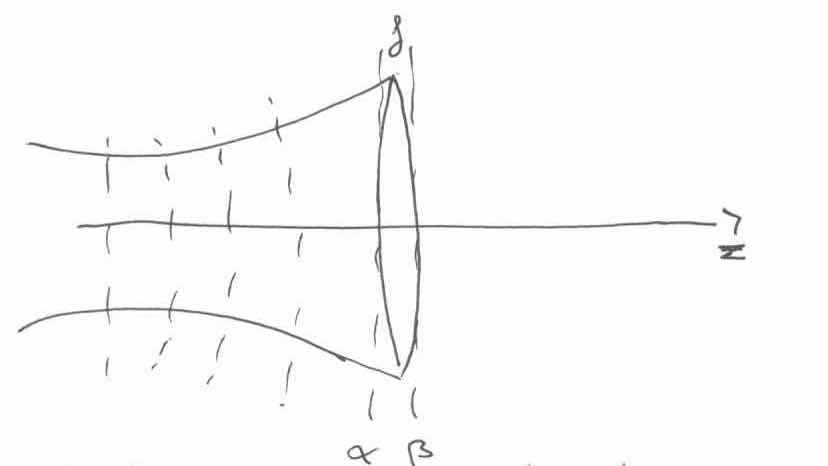
\includegraphics[height=4cm]{images/1}
\end{figure}
Detti $q_\alpha$ e $q_\beta$ i parametri complessi del fascio gaussiano appena prima e appena dopo la lente, per la legge ABCD
\begin{equation*}
q_\beta = \frac{Aq_\alpha + B}{Cq_\alpha + D} \quad \text{con} \quad
\begin{bmatrix}
1	&	0\\
-\frac{1}{f}	&	1
\end{bmatrix}
\end{equation*}
e quindi:
\begin{equation*}
q_\beta = \frac{q_\alpha}{-\frac{1}{f}q_\alpha + 1}
\end{equation*}
Ricordando l'Ansatz: $\frac{1}{q} = \frac{1}{R} -i\frac{\l}{\pi \w^2}$, ho
\begin{equation*}
\frac{1}{R_\beta} -i\frac{\l}{\pi\omega_beta^2} = \frac{1}{R_\alpha} -i\frac{\l}{\pi \omega_\alpha^2} - \frac{1}{f}
\end{equation*}
Uguagliando la parte reale e la parte immaginaria ho infine:
\begin{equation*}
\begin{cases}
\frac{1}{R_\beta} \frac{1}{R_\alpha} - \frac{1}{f}\\
w_\beta = w_\alpha
\end{cases}
\end{equation*}
cioè la lente sottile non modifica lo spot-size del fascio gaussiano mentre ne modifica il suo raggio di curvatura.
\begin{figure}[H]
\centering
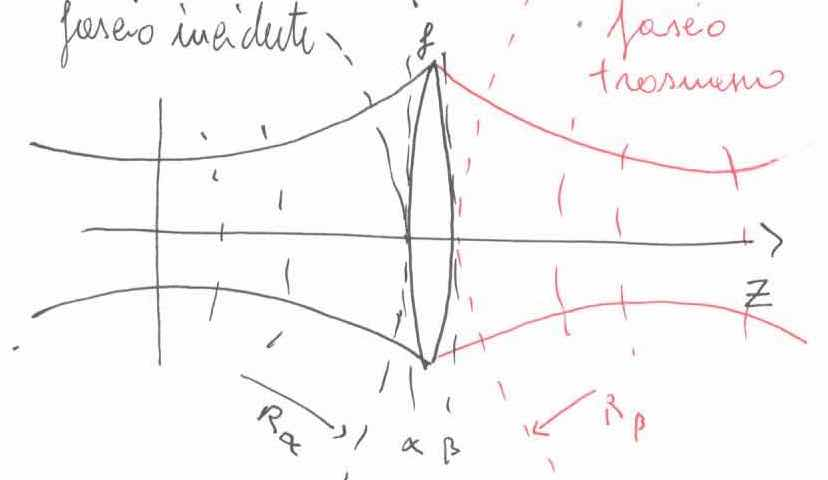
\includegraphics[height=4cm]{images/2}
\end{figure}

2) Focalizzazione di un fascio gaussiano
\begin{figure}[H]
\centering
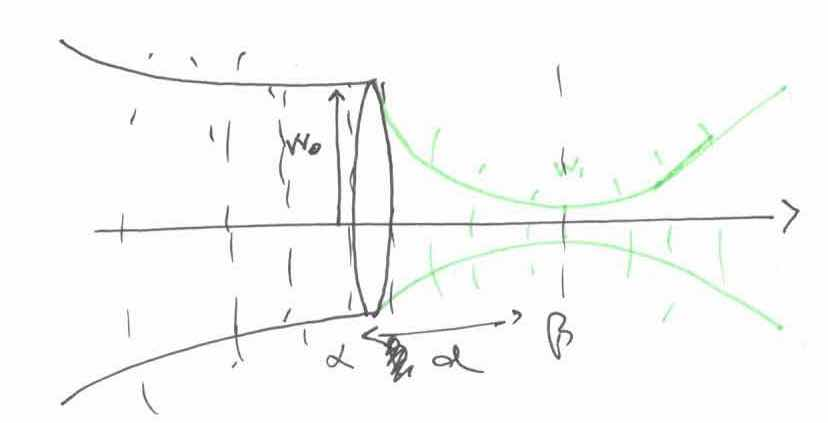
\includegraphics[height=4cm]{images/3}
\end{figure}
Siano $\alpha$ e $\beta$ i piani di figura. Per costruzione $q_\alpha = izR_\alpha =i\frac{\pi w_0^2}{\l}$ e $q_\beta = izR_\beta = i\frac{\pi w_1^2}{\l}$.
Inoltre, per la legge ABCD:
\begin{equation*}
q_\beta = \frac{Aq_\alpha + B}{Cq_\alpha + D} \quad \text{con} \quad
\begin{bmatrix}
1	&	d\\
0	&	1
\end{bmatrix} \begin{bmatrix}
1	&	0\\
-\frac{1}{f}	&	1
\end{bmatrix}
=
\begin{bmatrix}
1-\frac{d}{f}	&	d\\
-\frac{1}{f}	&	1
\end{bmatrix}
\end{equation*}
Pertanto:
\begin{equation*}
iz_{R_\beta} = \frac{iz_{R_\alpha A + B}}{iz_{R\alpha C + D}}\quad -z_{R_\alpha} z_{R_\beta} C +iDz_{R_\beta} = iDz_{R_\alpha} + B
\end{equation*}
Uguagliando la parte reale e immaginaria:
\begin{equation*}
\begin{cases}
z_{R_\alpha} z_{R_\beta} C = -B\\
D z_{R_\beta} = A z_{R\alpha} \rightarrow z_{R_\beta = \frac{A}{D} z_{R\alpha}}
\end{cases}
\end{equation*}
Dalla seconda equazione $z_{R_\beta} = \frac{A}{D} z_{R_\alpha}$, e quindi
\begin{equation*}
z_{R_\alpha}^2 \frac{A}{D} C = -B
\end{equation*}
ovvero:
\begin{equation*}
z_{R_\alpha}^2 \left(1 - \frac{d}{f}\right) \left(-\frac{1}{f}\right) = d
\end{equation*}
quindi:
\begin{align*}
d &= \frac{z_{R_\alpha}^2}{f + \frac{z_{R_\alpha}^2}{f}}\\
&= \frac{f}{1 + \left(\frac{f}{z_{R_\alpha}}\right)^2}
\end{align*}
\begin{equation*}
z_{R_\alpha} = \frac{A}{D}z_{R_\alpha} = 1 - \frac{d}{f} z_{R_\alpha} = \left[ 1 - \frac{1}{1 + \left( \frac{f}{z_{R_\alpha}}\right)}\right] z_{R_\alpha}
\end{equation*}
\begin{equation*}
w_1 = \sqrt{\frac{\left(\frac{f}{z_{R_\alpha}}\right)^2}{1 + \left( \frac{f}{z_{R_\alpha}}\right)^2}} w_0
\end{equation*}
Nel limite $z_R >> f$, ho $d \simeq f$ e $w_1 \simeq w_0 \frac{f}{\frac{\pi w_0^2}{\l}} = \frac{\l}{\pi w_0}f = \theta_d f$ essendo $\theta_d \equiv \frac{\l}{\pi w_0}$ è l'angolo di divergenza del fascio gaussiano incidente.
Interpretazione fisica:
\begin{figure}[H]
\centering
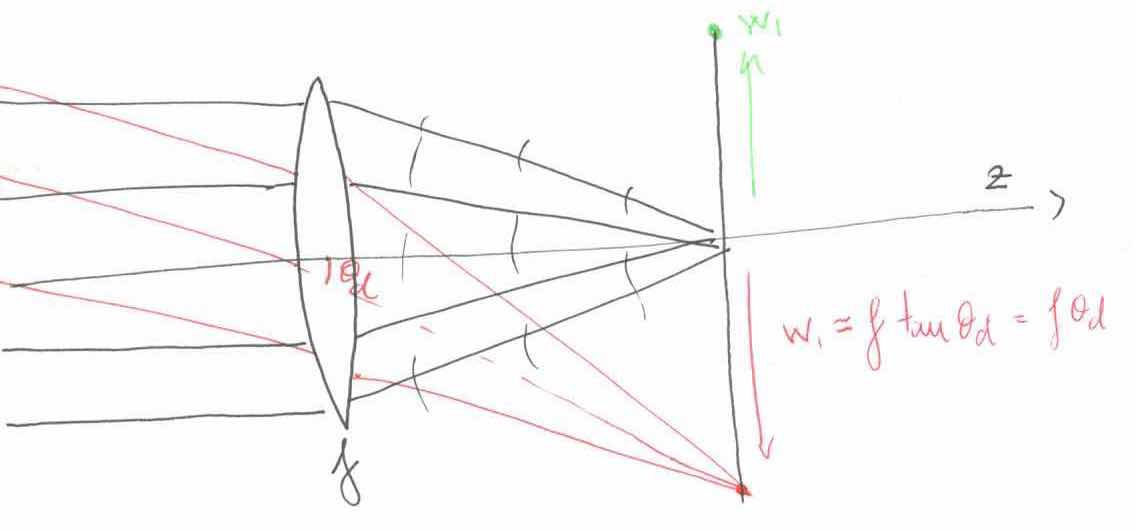
\includegraphics[height=4cm]{images/4}
\end{figure}

3) Legge dei punti coniugati per i fasci gaussiani
\begin{figure}[H]
\centering
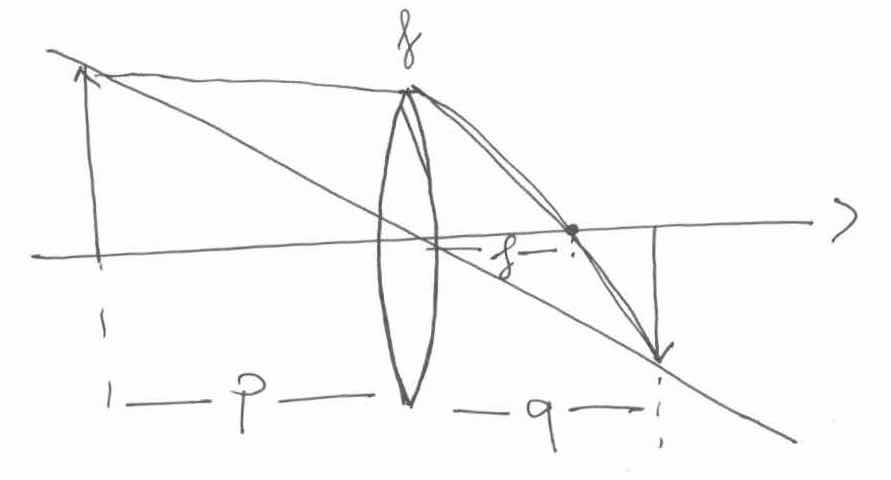
\includegraphics[height=4cm]{images/5}
\end{figure}
Consideriamo $q$ e $w_1$ dato $p$, $w_0$ e $f$ nel seguente problema
\begin{figure}[H]
\centering
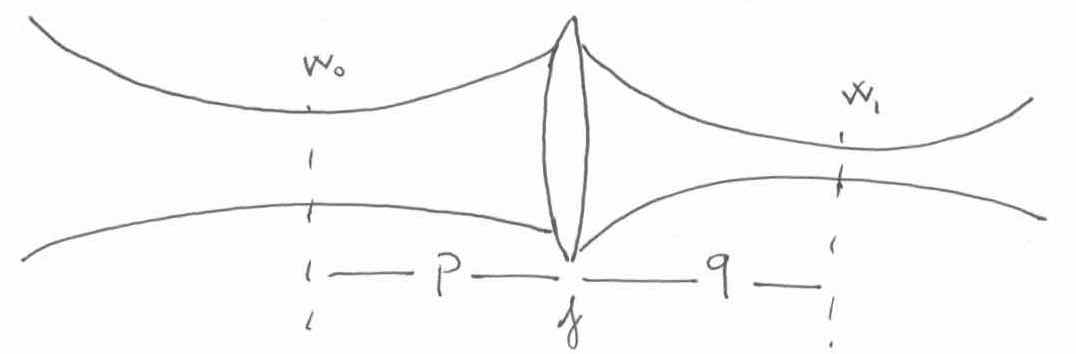
\includegraphics[height=4cm]{images/6}
\end{figure}
Detti $\alpha$ e $\beta$ i piani dei beam waist di figura, per costruzione: $q_\alpha = izR_\alpha =i\frac{\pi w_0^2}{\l}$ e $q_\beta = izR_\beta = i\frac{\pi w_1^2}{\l}$.
Inoltre, per la legge ABCD
\begin{equation*}
q_\beta = \frac{Aq_\alpha + B}{Cq_\alpha + D} \quad \text{con} \quad
\begin{bmatrix}
1	&	q\\
0	&	1
\end{bmatrix} \begin{bmatrix}
1	&	0\\
-\frac{1}{f}	&	1
\end{bmatrix} \begin{bmatrix}
1	&	p\\
0	&	1
\end{bmatrix}
=
\begin{bmatrix}
1-\frac{q}{f}	&	p + q - \frac{pq}{f}\\
-\frac{1}{f}	&	1 - \frac{p}{f}
\end{bmatrix}
\end{equation*}
da cui
\begin{equation*}
iz_{R_\beta} = \frac{iz_{R_\alpha A + B}}{iz_{R\alpha C + D}}\quad -z_{R_\alpha} z_{R_\beta} C +iDz_{R_\beta} = iDz_{R_\alpha} + B
\end{equation*}
uguagliando parte $\Re$ e parte $\Im$ ho
\begin{equation*}
\begin{cases}
-z_{R_\alpha} z_R{\beta} C = B\\
z_{R_\beta} D = A z_{R_\alpha}
\end{cases}
\end{equation*}
Risulta
\begin{equation*}
\frac{1}{q} = \frac{1}{f} - \frac{1}{p} \frac{1}{1 + \frac{z_{R_\alpha}}{p(p-f)}}
\end{equation*}
\begin{equation*}
w_1 = \left|\frac{q}{p}\right| \frac{w_0}{\sqrt{\frac{q}{p} + \left[ 1 + \frac{z_{R_\alpha}}{p(p-f)}\right] \left(	1 - \frac{q}{p}\right)}}
\end{equation*}
%\begin{oss}
\begin{enumerate}
\item Considerando i limite di fascio gaussiano incidente che tende ad un'onda sferica, cioè $z_{R_\alpha} = \frac{\pi w_0^2}{\l} \rightarrow 0$, e $p \neq f$, $p \neq 0$; in tal caso si ha:
\begin{equation*}
\frac{1}{q} \simeq \frac{1}{f} - \frac{1}{p}
\end{equation*}
che è la legge dei punti coniugati dell'ottica geometrica. In tale limite, inoltre
\begin{equation*}
w_1 \simeq \left|\frac{q}{p}\right| w_0
\end{equation*}
che è la legge ordinaria con rapporto d'ingrandimento $M= \left| \frac{q}{p}\right|$.
\item Si consideri il caso $p = f$. In tal caso $q \simeq f$
\end{enumerate}


Tema d'esame 3 Luglio 2009
Si consideri il sistema ottico in figura:
\begin{figure}[H]
\centering
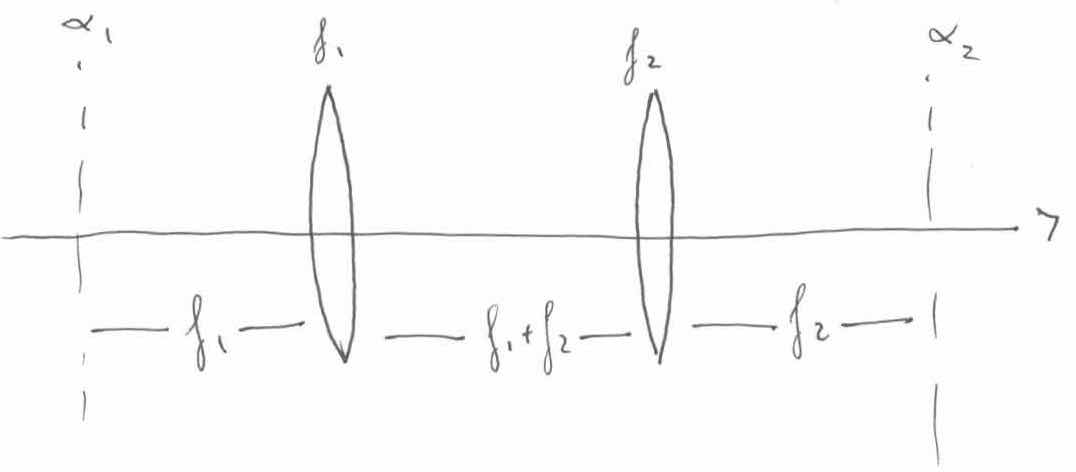
\includegraphics[height=4cm]{images/7}
\end{figure}
1) Calcolare la matrice da $\alpha_1 \rightarrow \alpha_2$:
\begin{equation*}
\begin{bmatrix}
1	&	f_2\\
0	&	1
\end{bmatrix}
\begin{bmatrix}
1	&	0\\
-\frac{1}{f_2}	&	1
\end{bmatrix}
\begin{bmatrix}
1	&	f_1 + f_2\\
0	&	1
\end{bmatrix}
\begin{bmatrix}
1	&	0\\
-\frac{1}{f_1}	&	1
\end{bmatrix}
\begin{bmatrix}
1	&	f_1\\
0	&	1
\end{bmatrix}
=
\begin{bmatrix}
-\frac{f_2}{f_1}	&	0\\
0	&	- \frac{f_1}{f_2}
\end{bmatrix}
\end{equation*}
Usando la legge ABCD si ha che:
\begin{equation*}
q_2 = \frac{Aq_1 + B}{Cq_1 + D}
\end{equation*}
essendo $q_1 + q_2$ i parametri complessi del fascio gaussiano ai piani $\alpha_1$ e $\alpha_2$.
Ricordando l'Ansatz:
$\frac{1}{q_1} = \frac{1}{R_1} -i\frac{\l}{\pi w_1^2}$ e $\frac{1}{q_2} = \frac{1}{R_2} -i\frac{\l}{\pi w_2^2}$ ottengo $q_2 = \frac{A}{D}q_1$, $\frac{1}{q_2} = \frac{D}{A}\frac{1}{q_1}$, ovvero $\frac{1}{R_2} -i\frac{\l}{\pi w_2^2} = \left(\frac{f_1}{f_2}\right)^2 \left[\frac{1}{R_1} - i\frac{\l}{\pi w_1^2}\right]$.
Uguagliando parte reale e parte immaginaria si ha
\begin{equation*}
\begin{cases}
R_2 = \left(\frac{f_2}{f_1}\right)^2 R_1\\
w_2 = \left|\frac{f_1}{f_2}\right|w_1
\end{cases}
\end{equation*}